\chapter{Polynomial Approximation}
\label{appendix:a}
\section{Piece-wise Polynomial Periodic Function}
\label{section:piecewise_periodic_polynomial}
To make each Newton's method iteration more computationally efficient, and to simplify the gradient and Hessian derivations and the technical implementation details in general, we design a smooth periodic function $f_p: \mathbb{R} \xrightarrow[]{} \mathbb{R}$ with period $p$, that satisfies the following requirements for any $x \in \mathbb{R}$ and $k \in \mathbb{Z}$:
\begin{equation}\label{eq:periodic_req}
\begin{split}
&0 \leq f_p\left(x\right) \leq 1 \\
&f_p\left(x\right) = f_p\left(x + kp\right) \\
&f_p\left(\frac{p}{2} + kp\right) = 1 \\
&f_p\left(kp\right) = 0 \\
\end{split}
\end{equation}
In other words, we simply want its roots to be periodic. We achieve it by finding a polynomial $g\left(x\right)$ that satisfies requirements \ref{eq:periodic_req} in the interval $\left[0, p\right]$, and replicating it over the whole real-numbers domain. Explicitly, we want the polynomial to satisfy the following:
\begin{equation}\label{eq:system_of_equations}
\begin{split}
&g\left(0\right) = 0, \quad,
g\left(\frac{p}{2}\right) = 1, \quad,
g\left(p\right) = 0 \\ \\
&\frac{dg}{dx}\left(0\right) = 0, \quad
\frac{dg}{dx}\left(\frac{p}{2}\right) = 0, \quad
\frac{dg}{dx}\left(p\right) = 0
\end{split}
\end{equation}
This suggest that $g\left(x\right)$ is a polynomial of degree 6. Therefore, $g\left(x\right)$ is given by:
\begin{equation}\label{eq:polynomial_6}
\begin{split}
g\left(x\right) = a_0 + a_1x + a_2x^2 + a_3x^3 + a_4x^4 + a_5x^5 = a^T \cdot \mathrm{x}\left(x\right)
\end{split}
\end{equation}
Where $a = \left(a_0,a_1,a_2,a_3,a_4,a_5\right)^T$ and $\mathrm{x}\left(x\right) = \left(1,x,x^2,x^3,x^4,x^5\right)^T$.
Solving the linear system of equations \ref{eq:system_of_equations} yields the desired coefficients vector $a_* = \left(a^*_0,a^*_1,a^*_2,a^*_3,a^*_4,a^*_5\right)^T$. Therefore, we define $f_p\left(x\right)$ as follows:
\begin{equation}\label{eq:polynomial_6}
\begin{split}
f_p\left(x\right) = 
\begin{cases} 
  g_*\left(x\right) & x \in \left[0,p\right] \\
  g_*\left(x \mod{p}\right) & x \notin \left[0,p\right]
\end{cases}
\end{split}
\end{equation}
Where $g_*\left(x\right) = a_*^T \cdot \mathrm{x}\left(x\right)$. We call $f_p\left(x\right)$ a \emph{piece-wise polynomial periodic function}. Figure \ref{fig:polynomial_periodic_function} visualize $f_p\left(x\right)$ for an arbitrary period.
\begin{figure}[ht]
\centering
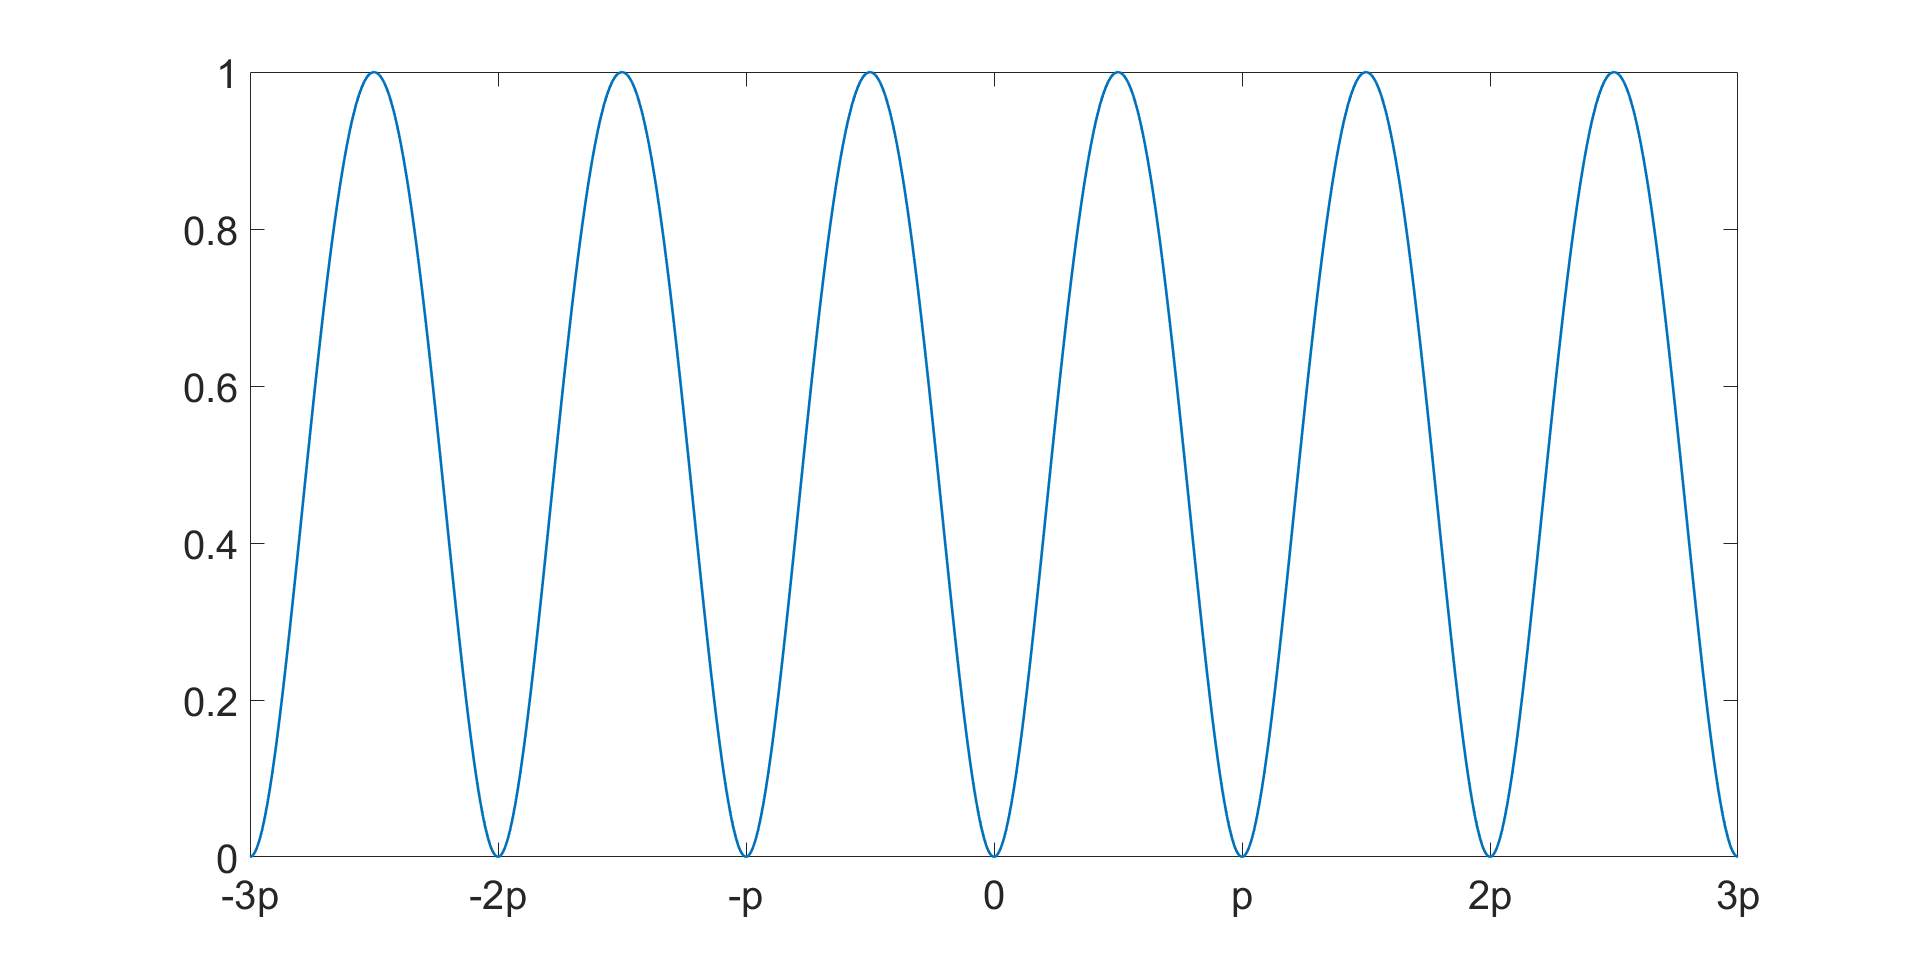
\includegraphics[width=12cm]{figures/periodic_function.png}
\caption[Piece-wise Polynomial Periodic Function]{A plot of $f_p\left(x\right)$ in the interval $\left[-3p, 3p\right]$. As can be seen, $f_p\left(x\right)$ is a priodic function, where its roots are equally spaced with a distance $p$.}
\label{fig:polynomial_periodic_function}
\end{figure}
\section{First Derivative}
The first derivative of $g_*\left(x\right)$ is given by:
\begin{equation}\label{eq:polynomial_6}
\begin{split}
g'_*\left(x\right) = a^*_1 + 2a^*_2x + 3a^*_3x^2 + 4a^*_4x^3 + 5a^*_5x^4 = b_*^T \cdot \mathrm{x}\left(x\right)
\end{split}
\end{equation}
Where $b_* = \left(a^*_1,2a^*_2,3a^*_3,4a^*_4,5a^*_5,0\right)^T$ and $\mathrm{x}\left(x\right) = \left(1,x,x^2,x^3,x^4,x^5\right)^T$. Therefore, we define $f'_p\left(x\right)$ is given as follows:
\begin{equation}\label{eq:polynomial_6}
\begin{split}
f'_p\left(x\right) = 
\begin{cases} 
  g'_*\left(x\right) & x \in \left[0,p\right] \\
  g'_*\left(x \mod{p}\right) & x \notin \left[0,p\right]
\end{cases}
\end{split}
\end{equation}
\section{Second Derivative}
The second derivative of $g_*\left(x\right)$ is given by:
\begin{equation}\label{eq:polynomial_6}
\begin{split}
g''_*\left(x\right) = 2a^*_2 + 6a^*_3x + 12a^*_4x^2 + 20a^*_5x^3 = c_*^T \cdot \mathrm{x}\left(x\right)
\end{split}
\end{equation}
Where $c_* = \left(2a^*_2,6a^*_3, 12a^*_4,20a^*_5,0,0\right)^T$ and $\mathrm{x}\left(x\right) = \left(1,x,x^2,x^3,x^4,x^5\right)^T$. Therefore, we define $f''_p\left(x\right)$ is given as follows:
\begin{equation}\label{eq:polynomial_6}
\begin{split}
f''_p\left(x\right) = 
\begin{cases} 
  g''_*\left(x\right) & x \in \left[0,p\right] \\
  g''_*\left(x \mod{p}\right) & x \notin \left[0,p\right]
\end{cases}
\end{split}
\end{equation}
\chapter{Gradient and Hessian Derivations}
In this appendix, we show detailed derivations for the gradient and Hessian of each individual penalty function, as defined in chapter \ref{chapter:method}.
\section{Composition - General Case}
\label{section:composition_general_case}
Given two smooth functions $f: \mathbb{R}^m \xrightarrow[]{} \mathbb{R}$ and $h: \mathbb{R}^n \xrightarrow[]{} \mathbb{R}^m$, we derive the gradient and Hessian of their composition $g\left(x\right) = f \circ h \left(x\right)$.
\subsection{Gradient}
The differential of  $g\left(x\right)$ is computed as follows:
\begin{flalign}
dg\left(x\right) &= d\bigg(f\Big(h\left(x\right)\Big)\bigg) \\ &= \nabla f\Big(h\left(x\right)\Big)^T \cdot dh\left(x\right)
\\
& = \nabla f \Big(h\left(x\right)\Big)^T \cdot J_h\left(x\right) \cdot dx
\\
& = \bigg(J_h\left(x\right)^T \cdot \nabla f\Big(h\left(x\right)\Big)\bigg)^T \cdot dx \label{eq:generalized_composition_gradient}
\end{flalign}
By \ref{eq:generalized_composition_gradient} we get that the gradient $\nabla g\left(x\right)$ is given by:
\begin{flalign}
\nabla g\left(x\right) = J_h\left(x\right)^T \cdot \nabla f\Big(h\left(x\right)\Big)
\end{flalign}
Where $J_h\left(x\right)$ is the Jacobian matrix of $h$ at $x$.
\subsection{Hessian}
The differential of $\nabla g\left(x\right)$ is computed as follows:
\begin{flalign}
d \nabla g \left(x\right) &= d\bigg( J_h\left(x\right)^T \cdot \nabla f\Big(h\left(x\right)\Big) \bigg)
\\
&= d J_h\left(x\right)^T \cdot \nabla f\Big(h\left(x\right)\Big) + J_h\left(x\right)^T \cdot d \nabla f\Big(h\left(x\right)\Big)
\\
&= \Big(d J_h\left(x\right)\Big)^T \cdot \nabla f\Big(h\left(x\right)\Big) + J_h\left(x\right)^T \cdot d \nabla f\Big(h\left(x\right)\Big)
\\
&= \Big(T_h\left(x\right)dx\Big)^T \cdot \nabla f\Big(h\left(x\right)\Big) + J_h\left(x\right)^T \cdot \nabla^2 f\Big(h\left(x\right)\Big) \cdot dh\left(x\right)
\\
&= dx^T \cdot T_h\left(x\right)^T \cdot \nabla f\Big(h\left(x\right)\Big) + J_h\left(x\right)^T \cdot \nabla^2 f\Big(h\left(x\right)\Big) \cdot J_h\left(x\right) \cdot dx
\\
&= \bigg(T_h\left(x\right)^T \cdot \nabla f\Big(h\left(x\right)\Big)\bigg)^T \cdot dx + J_h\left(x\right)^T \cdot \nabla^2 f\Big(h\left(x\right)\Big) \cdot J_h\left(x\right) \cdot dx
\\
&= \underbrace{\nabla f\Big(h\left(x\right)\Big)^T \cdot T_h\left(x\right)}_{\text{$n \times n$ matrix}} \cdot dx + \underbrace{J_h\left(x\right)^T \cdot \nabla^2 f\Big(h\left(x\right)\Big) \cdot J_h\left(x\right)}_{\text{$n \times n$ matrix}} \cdot dx
\\
&= \bigg( \nabla f\Big(h\left(x\right)\Big)^T \cdot T_h\left(x\right) + J_h\left(x\right)^T \cdot \nabla^2 f\Big(h\left(x\right)\Big) \cdot J_h\left(x\right) \bigg) \cdot dx
\label{eq:generalized_composition_hessian}
\end{flalign}
By \ref{eq:generalized_composition_hessian} we get that the Hessian $\nabla^2 g\left(x\right)$ is given by:
\begin{flalign}
\nabla^2 g \left(x\right) = \nabla f\Big(h\left(x\right)\Big)^T \cdot T_h\left(x\right) + J_h\left(x\right)^T \cdot \nabla^2 f\Big(h\left(x\right)\Big) \cdot J_h\left(x\right)
\end{flalign}
Where $T_h\left(x\right)$ is a tensor of $n$ matrices, each of size $m \times n$.
\subsection{Derivation of $T_h\left(x\right)$}
Let the components of $h\left(x\right)$ be defined as follows:
\begin{flalign}
    h\left(x\right) &= \begin{bmatrix}
           h_1\left(x\right) \\
           \vdots \\
           h_m\left(x\right)
         \end{bmatrix}
\end{flalign}
Such that $h_i\left(x\right): \mathbb{R}^n \xrightarrow[]{} \mathbb{R}$ for $i \in \left\{1,2,\hdots,m\right\}$. Using that explicit definition of $h\left(x\right)$, we get that the Jacobian $J_h\left(x\right)$ is given by:
\begin{flalign}
    J_h\left(x\right) &= \begin{bmatrix}
           \nabla h_1\left(x\right)^T \\
           \vdots \\
           \nabla h_m\left(x\right)^T
         \end{bmatrix}
\end{flalign}
The differential of $J_h\left(x\right)$ is given as follows:
\begin{flalign}
    dJ_h\left(x\right) &= \begin{bmatrix}
           d\nabla h_1\left(x\right)^T \\
           \vdots \\
           d\nabla h_m\left(x\right)^T
         \end{bmatrix}
\\
    &= \begin{bmatrix}
               \Big(d\nabla h_1\left(x\right)\Big)^T \\
               \vdots \\
               \Big(d\nabla h_m\left(x\right)\Big)^T
             \end{bmatrix}
\\
    &= \begin{bmatrix}
               \Big(\nabla^2 h_1\left(x\right) \cdot dx\Big)^T \\
               \vdots \\
               \Big(\nabla^2 h_m\left(x\right) \cdot dx\Big)^T
             \end{bmatrix}
\end{flalign}
Let $\mathrm{row}_i\Big(\nabla^2 h_j\left(x\right)\Big)$ be a function that returns the $i$th row of a given matrix. Let $M_i\left(x\right)$ be a matrix of size $m \times n$ defined as follows:
\begin{flalign}
    M_i\left(x\right) &=
    \begin{bmatrix}
       \mathrm{row}_i\Big(\nabla^2 h_1\left(x\right)\Big) \\
       \vdots \\
       \mathrm{row}_i\Big(\nabla^2 h_m\left(x\right)\Big) \\
    \end{bmatrix}
\end{flalign}
We now can rewrite $dJ_h\left(x\right)$ as follows:
\begin{flalign}
    dJ_h\left(x\right) &=
    \begin{bmatrix}
       M_1\left(x\right) dx & \hdots & M_n\left(x\right) dx
    \end{bmatrix}
    \\
    &= 
    \begin{bmatrix}
       M_1\left(x\right) & \hdots & M_n\left(x\right)
    \end{bmatrix} dx \\
    &= 
    T_h\left(x\right) dx
\end{flalign}
Where $T_h\left(x\right) = \begin{bmatrix} M_1\left(x\right) & \hdots & M_n\left(x\right) \end{bmatrix}$.
\section{Composition - Degenerate Case}
Even though the following derivation is a private case of \ref{section:composition_general_case}, we include it as well for clarity. Given two smooth functions $f: \mathbb{R} \xrightarrow[]{} \mathbb{R}$ and $h: \mathbb{R}^n \xrightarrow[]{} \mathbb{R}$, we derive the gradient and Hessian of their composition $f \circ h\left(x\right)$.
\subsection{Gradient}
The differential of  $f\Big(h\left(x\right)\Big)$ is computed as follows:
\begin{flalign}
df\Big(h\left(x\right)\Big) &= f'\Big(h\left(x\right)\Big) \cdot dh\left(x\right)
\\
& = f'\Big(h\left(x\right)\Big) \cdot \nabla h\left(x\right)^T \cdot dx
\\
& = \bigg(f'\Big(h\left(x\right)\Big) \cdot \nabla h\left(x\right)\bigg)^T \cdot dx \label{eq:composition_gradient}
\end{flalign}
By \ref{eq:composition_gradient} we get that the gradient $\nabla f\Big(h\left(x\right)\Big)$ is given by:
\begin{flalign}
\nabla f\Big(h\left(x\right)\Big) = f'\Big(h\left(x\right)\Big) \cdot \nabla h\left(x\right)
\end{flalign}
\subsection{Hessian}
The differential of  $\nabla f\Big(h\left(x\right)\Big)$ is computed as follows:
\begin{flalign}
d \nabla f\Big(h\left(x\right)\Big) &= d\bigg( f'\Big(h\left(x\right)\Big) \cdot \nabla h\left(x\right)\bigg)
\\
& = df'\Big(h\left(x\right)\Big) \cdot \nabla h\left(x\right) + f'\Big(h\left(x\right)\Big) \cdot d\nabla h\left(x\right)
\\
& = f''\Big(h\left(x\right)\Big) \cdot dh\left(x\right) \cdot \nabla h\left(x\right) + f'\Big(h\left(x\right)\Big) \cdot \nabla^2 h\left(x\right) \cdot dx
\\
& = f''\Big(h\left(x\right)\Big) \cdot \underbrace{\nabla h\left(x\right)^T \cdot dx}_{\text{scalar}} \cdot \nabla h\left(x\right) + f'\Big(h\left(x\right)\Big) \cdot \nabla^2 h\left(x\right) \cdot dx
\\
& = f''\Big(h\left(x\right)\Big) \cdot \underbrace{\nabla h\left(x\right) \cdot \nabla h\left(x\right)^T}_{\text{matrix}} \cdot dx + f'\Big(h\left(x\right)\Big) \cdot \nabla^2 h\left(x\right) \cdot dx
\\
& = \bigg(f''\Big(h\left(x\right)\Big) \cdot \nabla h\left(x\right) \cdot \nabla h\left(x\right)^T + f'\Big(h\left(x\right)\Big) \cdot \nabla^2 h\left(x\right)\bigg) \cdot dx
\label{eq:composition_hessian}
\end{flalign}
By \ref{eq:composition_hessian} we get that the Hessian $\nabla^2 f\Big(h\left(x\right)\Big)$ is given by:
\begin{flalign}
\nabla^2 f\Big(h\left(x\right)\Big) = f''\Big(h\left(x\right)\Big) \cdot \nabla h\left(x\right) \cdot \nabla h\left(x\right)^T + f'\Big(h\left(x\right)\Big) \cdot \nabla^2 h\left(x\right)
\end{flalign}
\section{Squared Norm}
\label{section:squared_norm}
In this section, we derive the gradient and Hessian of the squared Euclidean norm $g\left(x\right) = \norm{x}_2^2$, where $x \in \mathbb{R}^n$.
\subsection{Gradient}
The differential of $g\left(x\right)$ is computed as follows:
\begin{flalign}
dg\left(x\right) &= d\left(\norm{x}_2^2\right) \\
&= d\left(x^Tx\right) \\
&= \left(dx\right)^Tx + x^Tdx \\
&= x^Tdx + x^Tdx \\
&= 2x^Tdx \\
&= \left(2x\right)^Tdx
\label{eq:squared_norm_gradient}
\end{flalign}
By \ref{eq:squared_norm_gradient} we get that the gradient $\nabla g\left(x\right)$ is given by:
\begin{flalign}
\nabla \left(x\right) = 2x
\end{flalign}
\subsection{Hessian}
The differential of $\nabla g \left(x\right)$ is computed as follows:
\begin{flalign}
d \nabla g \left(x\right) &= d\left(2x\right) \\
&= 2dx \\
&= 2Idx
\label{eq:squared_norm_hessian}
\end{flalign}
By \ref{eq:squared_norm_hessian} we get that the gradient $\nabla^2 g\left(x\right)$ is given by:
\begin{flalign}
\nabla^2 g \left(x\right) = 2I
\end{flalign}
\section{\mathrb{atan2}}
\label{section:atan2}
In this section, we derive the gradient and Hessian of $\mathrm{atan2}\left(y,x\right)$, for $x,y \in \mathbb{R}$.
\subsection{Gradient}
It is \href{https://en.wikipedia.org/wiki/Atan2}{widely known} that the gradient $\nabla \mathrm{atan2}\left(y,x\right)$ is given by:
\begin{flalign}
\nabla \mathrm{atan2}\left(y,x\right) = \Big(-\frac{y}{x^2 + y^2}, \frac{x}{x^2 + y^2}\Big)
\end{flalign}
\subsection{Hessian}
Deriving the $2 \times 2$ Hessian matrix $\nabla^2 \mathrm{atan2}\left(y,x\right)$ is rather trivial, and is left as an exercise for the reader. 
\section{Angle Penalty Function}
\label{section:angle_penalty_function}
In paragraph \ref{paragraph:angle_penalty_function_method}, the angle penalty function was defined as follows:
\begin{equation}\label{eq:angle_penalty}
\begin{split}
P_{\mathrm{angle}}\left(e_i,e_j\right) = \mathrm{sin} \bigg( 4\Big(\theta\left(e_i\right) - \theta\left(e_j\right)\Big) - \frac{\pi}{2}\bigg) + 1
\end{split}
\end{equation}
Where $\theta\left(e_k\right) = \mathrm{atan2}\Big(\mathrm{y}\left(v_k^2\right) - \mathrm{y}\left(v_k^1\right), \mathrm{x}\left(v_k^2\right) - \mathrm{x}\left(v_k^1\right)\Big)$ is the angle formed by half-edge $e_k = \left(v^1_k, v^2_k\right)$ with the positive \emph{x-axis} direction, when treated as a vector based at $v_k^1$ and heading $v_k^2$, for $k \in \left\{i,j\right\}$.

\noindent By denoting:
\begin{equation}\label{eq:angle_penalty}
u = \Big(\mathrm{y}\left(v_i^2\right), \mathrm{y}\left(v_i^1\right), \mathrm{x}\left(v_i^2\right), \mathrm{x}\left(v_i^1\right), \mathrm{y}\left(v_j^2\right), \mathrm{y}\left(v_j^1\right), \mathrm{x}\left(v_j^2\right), \mathrm{x}\left(v_j^1\right)\Big)^T
\end{equation}
And by replacing the sine expression with a piece-wise polynomial periodic function $f_p$ with period $p=\frac{\pi}{2}$ (as defined in appendix \ref{appendix:a}), we can rewrite $P_{\mathrm{angle}}$ as follows:
\begin{equation}\label{eq:angle_penalty_rephrased}
\begin{split}
P_{\mathrm{angle}}\left(u\right) = f_{\frac{\pi}{2}} \bigg(h\left(u\right)\bigg)
\end{split}
\end{equation}
Where $h\left(u\right) = \mathrm{atan2}\Big(\delta_{0,1}\left(u\right), \delta_{2,3}\left(u\right)\Big) - \mathrm{atan2}\Big(\delta_{4,5}\left(u\right), \delta_{6,7}\left(u\right)\Big)$, and $\delta_{i,j}\left(u\right) = u_i - u_j$.

\noindent Since we already know how to calculate the first and second derivatives of $f_{\frac{\pi}{2}}$ (section \ref{section:piecewise_periodic_polynomial}), the gradient and Hessian of $\mathrm{atan2}$ (section \ref{section:atan2}), and we also know to calculate the gradient and Hessian of general composition of functions (section \ref{section:composition_general_case}), we only need to explicitly calculate $\nabla \delta_{i,j}\left(u\right)$ and $\nabla^2 \delta_{i,j}\left(u\right)$ in order to be able to calculate $\nabla P_{\mathrm{angle}}\left(u\right)$ and $\nabla^2 P_{\mathrm{angle}}\left(u\right)$.
\subsection{Deriving $\nabla \delta_{i,j}\left(u\right)$}
The differential of $\nabla \delta_{i,j}\left(u\right)$ is given by:
\begin{flalign}
d\nabla \delta_{i,j}\left(u\right) &= d\left(u_i - u_j\right) \\
&= \nabla u_i dx - \nabla u_j dx
\\
\label{delta_gradient}
&= \left(\nabla u_i - \nabla u_j\right) dx
\end{flalign}
Where $\nabla u_i$ and $\nabla u_j$ are one-hot vectors with 1 at index $i$ and $j$, respectively. By \ref{delta_gradient}, the gradient $\nabla \delta_{i,j}\left(u\right)$ is given by:
\begin{flalign}
\nabla \delta_{i,j}\left(u\right) = \nabla u_i - \nabla u_j
\end{flalign}
\subsection{Deriving $\nabla^2 \delta_{i,j}\left(u\right)$}
Since $\nabla \delta_{i,j}\left(u\right)$ is constant, we get that $\nabla^2 \delta_{i,j}\left(u\right) = 0$.
\section{Length Penalty Function}
In paragraph \ref{paragraph:length_penalty_function_method}, we defined the length penalty function $P_{length}$ as follows:
\begin{equation}\label{length_penalty}
\begin{split}
P_{\mathrm{length}}\left(e_i,e_j\right) = \left(\norm{e_i}_2^2 - \norm{e_j}_2^2\right)^2
\end{split}
\end{equation}
The length penalty measures the Euclidean length discrepancy between the two half-edges $e_i$ and $e_j$, where for $k \in \left\{i,j\right\}$, we have $e_k = \left(v^1_k, v^2_k\right)$. We can write $\norm{e_k}_2^2$ explicitly as follows:
\begin{flalign}
\norm{e_k}_2^2 &= \left(v^2_k - v^1_k\right)^T\left(v^2_k - v^1_k\right) \\
&= \Big(\mathrm{x}\left(v_k^2\right) - \mathrm{x}\left(v_k^1\right), \mathrm{y}\left(v_k^2\right) - \mathrm{y}\left(v_k^1\right) \Big)^T \Big(\mathrm{x}\left(v_k^2\right) - \mathrm{x}\left(v_k^1\right), \mathrm{y}\left(v_k^2\right) - \mathrm{y}\left(v_k^1\right) \Big)
\end{flalign}
\noindent By denoting:
\begin{equation}
u = \Big(\mathrm{y}\left(v_i^2\right), \mathrm{y}\left(v_i^1\right), \mathrm{x}\left(v_i^2\right), \mathrm{x}\left(v_i^1\right), \mathrm{y}\left(v_j^2\right), \mathrm{y}\left(v_j^1\right), \mathrm{x}\left(v_j^2\right), \mathrm{x}\left(v_j^1\right)\Big)^T
\end{equation}
we can write $\norm{e_i}_2^2$ and $\norm{e_j}_2^2$ as follows:
\begin{flalign}
\norm{e_i}_2^2 &= \Big(\delta_{2,3}\left(u\right), \delta_{0,1}\left(u\right)\Big)^T \Big(\delta_{2,3}\left(u\right), \delta_{0,1}\left(u\right)\Big)
\end{flalign}
\begin{flalign}
\norm{e_j}_2^2 &= \Big(\delta_{6,7}\left(u\right), \delta_{4,5}\left(u\right)\Big)^T \Big(\delta_{6,7}\left(u\right), \delta_{4,5}\left(u\right)\Big)
\end{flalign}
Where $\delta_{i,j}\left(u\right)$ is defined in section \ref{section:angle_penalty_function}.

\noindent Since we obviously know how to calculate the first and second derivatives of the square function of a real number, the gradient and Hessian of the squared norm (section \ref{section:squared_norm}), the gradient and Hessian of $\delta_{i,j}\left(u\right)$ (section \ref{section:angle_penalty_function}), and we also know to calculate the gradient and Hessian of general composition of functions (section \ref{section:composition_general_case}), we immediately know how to calculate $\nabla P_{\mathrm{length}}\left(u\right)$ and $\nabla^2 P_{\mathrm{length}}\left(u\right)$.
\section{Translation Penalty Function}
\label{section:translation_penalty_function}
In paragraph \ref{paragraph:translation_penalty_function_method}, we defined the translation penalty function $P_{\mathrm{translation}}$ as follows:
\begin{equation}\label{eq:translation_penalty}
\begin{split}
P_{\mathrm{translation}}\left(e_i,e_j\right) = \mathrm{sin} \Big( 2\pi\cdot\Delta_x\big(e_i,e_j\big) - \frac{\pi}{2}\Big) + \mathrm{sin} \Big( 2\pi\cdot\Delta_y\big(e_i,e_j\big) - \frac{\pi}{2}\Big) + 2
\end{split}
\end{equation}
Where $\Delta_x\big(e_i,e_j\big) = \mathrm{x}\left(v_i^1\right) - \mathrm{x}\left(v_j^1\right)$ and $\Delta_y\big(e_i,e_j\big) = \mathrm{y}\left(v_i^1\right) - \mathrm{y}\left(v_j^1\right)$ represent the Manhattan distance between the two twin-vertices $v^i_1$ and $v^j_1$, which is also, implicitly, the Manhattan distance between the two half-edges.

\noindent By denoting:
\begin{equation}\label{eq:angle_penalty}
u = \Big(\mathrm{y}\left(v_i^2\right), \mathrm{y}\left(v_i^1\right), \mathrm{x}\left(v_i^2\right), \mathrm{x}\left(v_i^1\right), \mathrm{y}\left(v_j^2\right), \mathrm{y}\left(v_j^1\right), \mathrm{x}\left(v_j^2\right), \mathrm{x}\left(v_j^1\right)\Big)^T
\end{equation}
And by replacing the sine expression with a piece-wise polynomial periodic function $f_p$ with period $p=1$ (as defined in appendix \ref{appendix:a}), we can rewrite $P_{\mathrm{translation}}$ as follows:
\begin{flalign}
P_{\mathrm{translation}}\left(u\right) = f_1\Big(\delta_{3,7}\left(u\right)\Big) + f_1\Big(\delta_{1,4}\left(u\right)\Big)
\end{flalign}
Where $\delta_{i,j}\left(u\right)$ is defined in section \ref{section:angle_penalty_function}.

\noindent Since we already know how to calculate the first and second derivatives of $f_1$ (section \ref{section:piecewise_periodic_polynomial}),  the gradient and Hessian of $\delta_{i,j}\left(u\right)$ (section \ref{section:angle_penalty_function}), and we also know to calculate the gradient and Hessian of general composition of functions (section \ref{section:composition_general_case}), we immediately know how to calculate $\nabla P_{\mathrm{translation}}\left(u\right)$ and $\nabla^2 P_{\mathrm{translation}}\left(u\right)$.
\section{Singular Points Penalty Function}
\label{section:singular_points_penalty_function_appendix}
In section \ref{section:singular_points_penlaty_function_method}, we defined the singular points penalty function $P_{\mathrm{singular}}\left(S\right)$ as follows:
\begin{equation}\label{eq:singular_points_penalty}
\begin{split}
P_{\mathrm{singular}}\left(S\right) = \sum_{v \in S} \bigg( \mathrm{sin} \Big( 2\pi\cdot\mathrm{x}\big(v\big) - \frac{\pi}{2}\Big) + \mathrm{sin} \Big( 2\pi\cdot\mathrm{y}\big(v\big) - \frac{\pi}{2}\Big) + 2 \bigg)
\end{split}
\end{equation}
Where $\mathrm{x}\big(u\big)$ and $\mathrm{y}\big(u\big)$ represent the domain coordinates of a twin-vertex in $S$.

\noindent By denoting:
\begin{equation}\label{eq:angle_penalty}
u = \Big(\mathrm{x}\left(v_0\right), \mathrm{y}\left(v_0\right), \mathrm{x}\left(v_1\right), \mathrm{y}\left(v_1\right), \hdots , \mathrm{x}\left(v_{\abs{S}-1}\right), \mathrm{y}\left(v_{\abs{S}-1}\right)\Big)^T
\end{equation}
And by replacing the sine expression with a piece-wise polynomial periodic function $f_p$ with period $p=1$ (as defined in appendix \ref{appendix:a}), we can rewrite $P_{\mathrm{singular}}$ as follows:
\begin{flalign}
P_{\mathrm{singular}}\left(u\right) = \sum_{i = 0}^{\abs{S} - 1} f_1\Big(\sigma_i\left(u\right)\Big)
\end{flalign}
Where $\sigma_i\left(u\right) = u_i$. Obviously, $\nabla \sigma_i\left(u\right)$ is the one-hot vector with 1 at index $i$, and $\nabla^2 \sigma_i\left(u\right) = 0$.

\noindent Since we already know how to calculate the first and second derivatives of $f_1$ (section \ref{section:piecewise_periodic_polynomial}),  the gradient and Hessian of $\sigma{i}\left(u\right)$, and we also know to calculate the gradient and Hessian of general composition of functions (section \ref{section:composition_general_case}), we immediately know how to calculate $\nabla P_{\mathrm{singular}}\left(u\right)$ and $\nabla^2 P_{\mathrm{singular}}\left(u\right)$.